\chapter{Results and Discussion}
This chapter presents and analyzes the results from experiments conducted on the simulation platform described previously.  
The chapter begins by reviewing the system's normal workflow in a standard scenario, which serves as a baseline for analysis.  
Subsequently, it introduces a more challenging ``user interplanetary mobility'' scenario.  
Through quantitative test data, this section reveals the performance limitations inherent in the current Johnson Draft when applied to this scenario.
Finally, based on an discussion of these limitations, the chapter offers a conceptual proposal to address the challenges.

\section{Baseline Scenario Review}

In its standard scenario, email transmission and reception rely entirely on the DTN gateway for relay.  
For instance, when a user on Earth sends an email to a user on the Moon, the message is submitted to the local \texttt{mail-1}.  
There, the \texttt{BPMailSend} gateway component encapsulates it into a bundle, which is then transmitted asynchronously and reliably over the DTN link to \texttt{mail-2}.  
Upon arrival, the \texttt{BPMailRecv} component decapsulates the bundle and delivers the email to the end user.  
In this scenario, interactive experience is seamless, as the high-latency interplanetary link is effectively shielded by the DTN gateway and the Bundle Protocol.

\section{User Interplanetary Mobility Scenario}

\subsection{Scenario Description and Problem Analysis}

A core assumption of existing DTN email gateway proposal is that the user's MUA and their home MTA/MDA are located within the same low-latency ``local'' network.  
However, this raises a practical and important question: how should users access their email when they travel between celestial bodies?

The key test scenario designed in this dissertation is as follows: a user whose home mailbox is on the Moon (located on \texttt{mail-2}) travels to Earth for a mission.  
From Earth, the user attempts to connect to and synchronize all the emails from their home server on the Moon using a local device (\texttt{client-1}).

In this scenario, a problem immediately becomes apparent.  
As depicted in Figure~\ref{fig:mobility_scenario}, the user's Thunderbird client is configured to connect directly to their home server \texttt{mail-2}.
Because \texttt{mail-2} is located on the distant Moon, this IMAP connection request must traverse the entire long-latency interplanetary link.  
The DTN gateway is completely bypassed in this process because IMAP is an end-to-end, TCP-based, real-time synchronization protocol that cannot be handled by an gateway like BPMail.


\begin{figure}[ht]
      \centering
      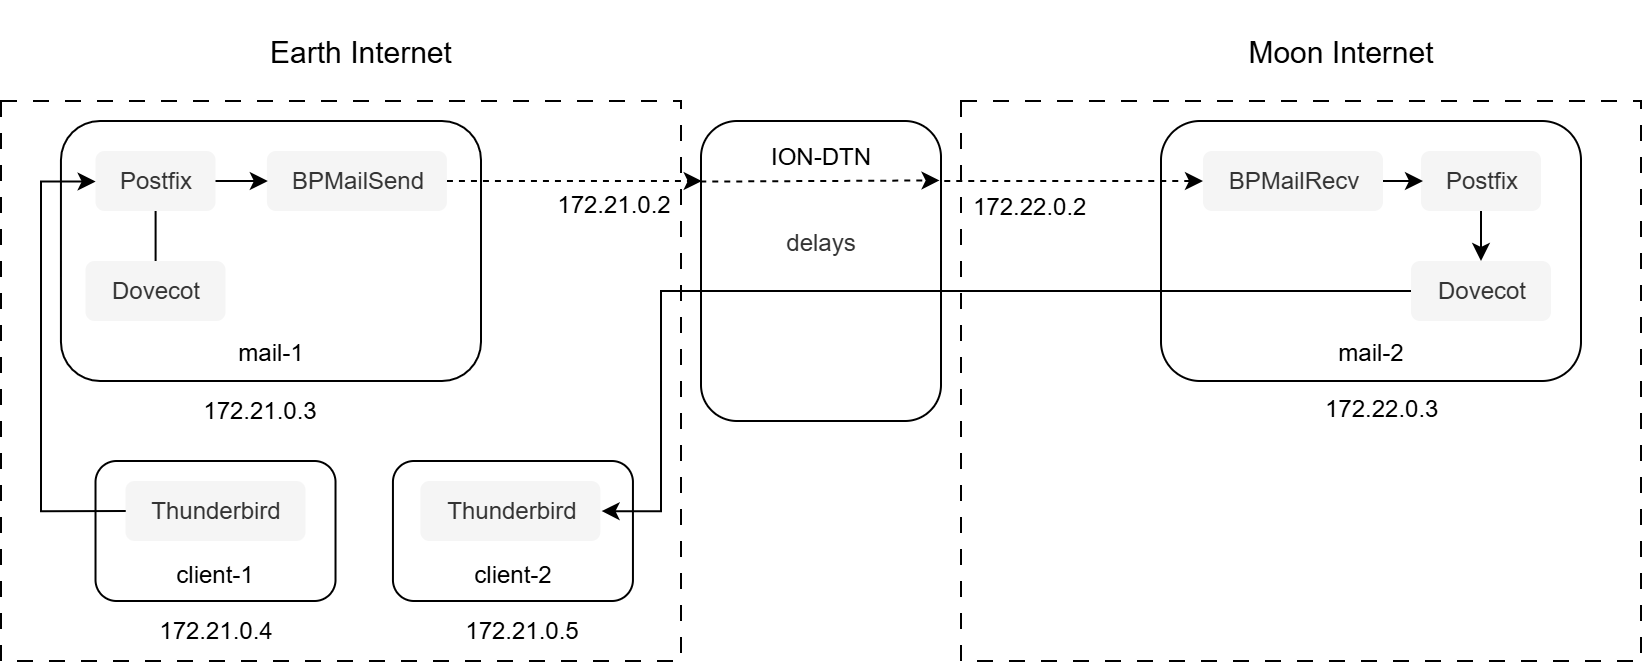
\includegraphics[width=1.0\textwidth]{Results/mobility_scenario.png}
      \caption{Illustration of the mobility scenario}
      \label{fig:mobility_scenario}
\end{figure}

\subsection{Experimental Results}
To quantify the impact of this problem, an experiment was conducted to measure the total time required for a client on Earth to synchronize 1000 simple emails (with the body ``Hello'') from the server on the Moon under various network delays.  
The results are presented in Table~\ref{tab:email-retrieval-time}.

\begin{table}[ht]
\centering
\setlength{\tabcolsep}{10pt}
\caption{Email retrieval time under different delays}
\label{tab:email-retrieval-time}
\begin{tabular}{cccc}
\hline
\textbf{Delay (s)} & \textbf{Body} & \textbf{Number of Emails} & \textbf{Retrieval Time (s)} \\
\hline
0   & "Hello" & 1000 & 19  \\
1   & "Hello" & 1000 & 33  \\
2   & "Hello" & 1000 & 64  \\
5   & "Hello" & 1000 & 153 \\
0   & "Hello" with attachment & 1 & Time out \\
\hline
\end{tabular}
\end{table}

As is clearly evident from Table~\ref{tab:email-retrieval-time}, the email retrieval time deteriorates sharply as the one-way delay increases.  
In a zero-delay environment (equivalent to a local area network), retrieving the emails takes only 19 seconds.  
However, when the delay reaches 5 seconds, completing the synchronization requires 153 seconds (over two and a half minutes).  
At this point, the user experience becomes unacceptable, and the system is rendered effectively unusable.

\section{Discussion and Limitation Analysis}

The experimental results above reveal multiple limitations in the design of the Johnson Draft.

\subsection{Architectural Limitation}

The data provides direct evidence of the proposal's failure to support user interplanetary mobility.  
The effectiveness of this solution is predicated on decoupling real-time user interaction (Client--Server) from asynchronous server-to-server relay (Server--Server) and applying DTN technology only to the latter.  
When a user roams, the client--server interaction, which is supposed to occur over a local, low-latency network, is forced to traverse a long-latency interplanetary link.  
This negates the delay-tolerant advantages of the entire system.  
The performance collapse is caused by ``chatty'' protocols like IMAP and SMTP, which require numerous round-trips that are severely penalized by high latency.

\subsection{Implementation Limitation}

During testing, a significant bottleneck was identified in the practical application of the current proposal: the BPMail gateway implementation is incapable of correctly processing emails with large attachments.

When attempting to send an email with a moderately large attachment (e.g., 3\,MB) through the gateway, the mail delivery fails.  
The likely cause of this issue lies within the memory management mechanisms of the BPMail software itself.  
For instance, the program may attempt to read the entire email content into a fixed-size memory buffer.  
When the email size exceeds this buffer's capacity, a buffer overflow or memory allocation failure occurs.

This implementation flaw severely limits the practical utility of the solution.  
In modern communication, email serves not only as a medium for text but also as a crucial tool for exchanging files and data.  
An email system that cannot handle a 3\,MB attachment is unacceptable for many real-world applications.



\section{Discussion of Extension}

To address the limitations identified above, particularly the challenges related to user mobility, this section proposes a conceptual extension informed by existing research in related fields.

In fact, the problem identified in this research falls under the broader category of ``Mobility Management'' within the field of DTN.  
Existing research has generally pursued solutions at two distinct layers:

\begin{itemize}
    \item \textbf{The Network Layer}: This approach aims to provide transparent mobility support through mechanisms such as dynamic routing protocols or directory services that track the changing locations of mobile nodes and route data accordingly.
    \item \textbf{The Application Layer}: This approach focuses on using proxies or caches to confine real-time user--service interactions to the local network, while handling data synchronization asynchronously in the background. Concepts like ``Data Mules'' are a classic example of this application-layer data ferrying philosophy.
\end{itemize}

Given the immense complexity of network-layer solutions, an application-layer proxy approach represents a more pragmatic and readily achievable path.
To this end, this dissertation proposes the \textit{On-demand Sync Agent} extension, a specific conceptualization of an application-layer solution.  
Its architecture is depicted in Figure~\ref{fig:sync_agent}.

\begin{figure}[ht]
      \centering
      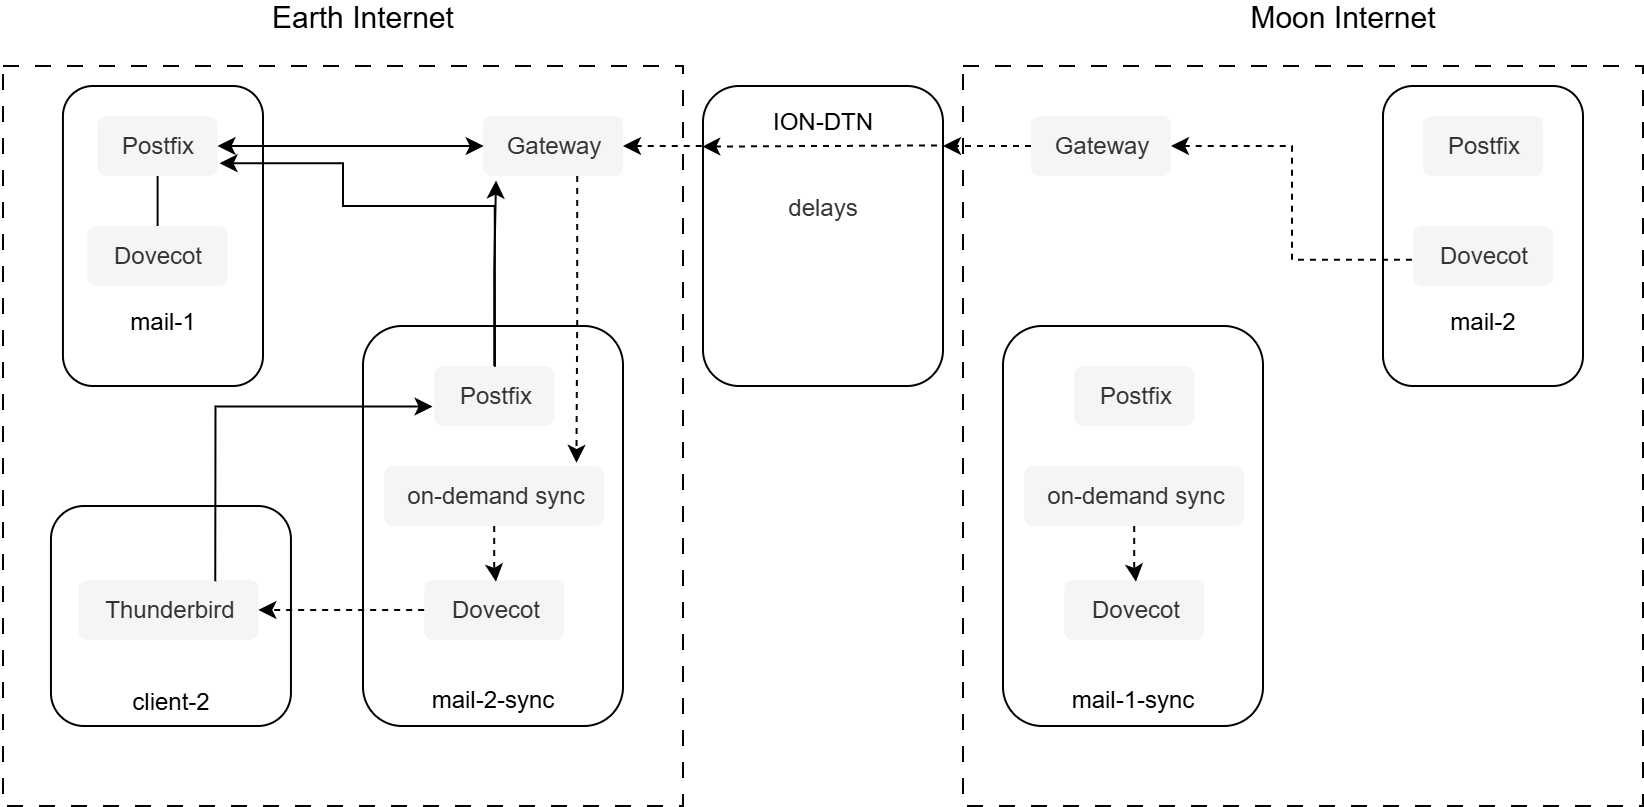
\includegraphics[width=1.0\textwidth]{Results/sync_agent.png}
      \caption{Conceptual Extension of the On-demand Sync Agent}
      \label{fig:sync_agent}
\end{figure}

The operational logic of this conceptual architecture is as follows:

\begin{enumerate}
    \item \textit{Introduction of a Local Sync Agent}: A ``Sync Agent'' service is deployed on each celestial body (e.g., Earth). To the user, this service appears as a fully functional, local mail server.
    \item \textit{Localization of User Interaction}: A roaming user (e.g., a user from the Moon who has traveled to Earth) configures their Thunderbird client to connect to this local Sync Agent on Earth, not to their distant home server on the Moon. This ensures a seamless and responsive user experience.
    \item \textit{Background DTN Synchronization}: The Sync Agent is responsible for conducting batch, asynchronous email synchronization with the user's home server (e.g., \texttt{mail-2} on the Moon) in the background. All data that must cross the interplanetary link is handled by the agent, which encapsulates it into bundles for transmission via the DTN gateway.
\end{enumerate}

This conceptual extension decouples the user's real-time interactions from the background data synchronization by introducing an intermediary proxy layer.
It thus holds potential to resolve the performance issues caused by user roaming.

It must be emphasized, however, that this is a preliminary architectural concept intended to inspire future research.  
It still faces significant challenges — for example, the proposed "Sync Agent" would require email service providers to pre-deploy servers on other planets, which poses considerable implementation difficulties.

\section{Summary}

By designing and testing a key ``user interplanetary mobility'' scenario, this chapter has identified and validated limitations of the existing DTN email gateway proposal.  

First, experimental data demonstrated that direct access to a remote mail server in a roaming scenario leads to severe performance degradation.  
Second, functional testing revealed that the core BPMail gateway component is unable to handle large attachments.  

Following a discussion of these limitations, this chapter proposed an extension based on an \textit{Sync Agent}, and revealed its shortcomings as well.
